% ============================================================
% fig_model_structure.tex — 论文 Fig. 1：Wendling 四群体微回路示意图
%
% 用途：替代原来的 structure.pdf（draw.io 导出：Arial 字体、四个方框形状不统一
%       ——椭圆/菱形/六边形，且没有可编辑源文件）。本文件是纯 TikZ，改文字、
%       箭头、配色都直接改这里，字体与正文一致。
%
% 编译：在 figures/ 目录下执行  pdflatex fig_model_structure.tex
%       → fig_model_structure.pdf（矢量，字体嵌入）
%
% 箭头含义（与论文 §3.1 正文一致）
%   PC → EIN / SIN / FIN    兴奋 (+)
%   EIN → PC                兴奋 (+)
%   SIN → PC                抑制 (−)
%   FIN → PC                抑制 (−)
%   SIN → FIN               抑制 (−)
%   虚线 p(t) → EIN         外部传入驱动，只加到兴奋性中间神经元上
%
% 排版：整幅约 10 cm × 5.5 cm，论文里按 0.78\textwidth 插入，
%       印刷后框内文字约 9.5 pt，与图注字号协调。
% ============================================================
\documentclass[border=4pt]{standalone}
\usepackage{tikz}
\usepackage{amsmath}
\usetikzlibrary{arrows.meta, calc}

\begin{document}
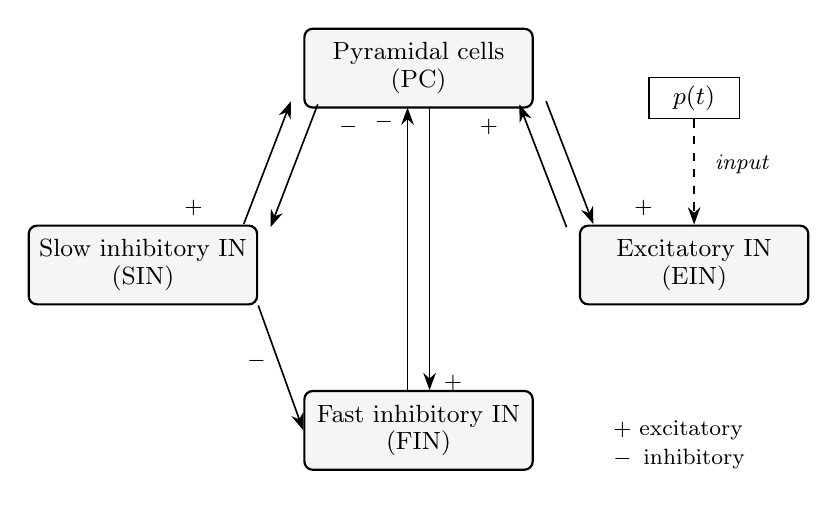
\begin{tikzpicture}[
    font=\small,
    >={Stealth[length=2.2mm, width=1.6mm]},
    pop/.style = {draw, rounded corners=3pt, thick,
                  minimum width=2.9cm, minimum height=1.0cm,
                  align=center, fill=black!4, inner sep=2pt},
    ar/.style  = {->, semithick},
    sg/.style  = {font=\footnotesize\bfseries, inner sep=1pt}
]

% ---------------- 四个群体 ----------------
\node[pop] (pc)  at (0,    3.00) {Pyramidal cells\\[-1pt](PC)};
\node[pop] (sin) at (-3.5, 0.50) {Slow inhibitory IN\\[-1pt](SIN)};
\node[pop] (ein) at (3.5,  0.50) {Excitatory IN\\[-1pt](EIN)};
\node[pop] (fin) at (0,   -1.60) {Fast inhibitory IN\\[-1pt](FIN)};

% ---------------- PC ↔ SIN（两条平行线） ----------------
\draw[ar] (-1.28,2.54) -- (-1.88,0.98);
\node[sg, anchor=east] at (-2.70,1.22) {$+$};
\draw[ar] (-2.22,1.02) -- (-1.62,2.58);
\node[sg, anchor=west] at (-1.05,2.25) {$-$};

% ---------------- PC ↔ EIN ----------------
\draw[ar] (1.62,2.58)  -- (2.22,1.02);
\node[sg, anchor=west] at (2.70,1.22) {$+$};
\draw[ar] (1.88,0.98)  -- (1.28,2.54);
\node[sg, anchor=east] at (1.05,2.25) {$+$};

% ---------------- PC ↔ FIN（竖直两条线） ----------------
\draw[ar] (0.14,2.50) -- (0.14,-1.09);
\node[sg, anchor=west] at (0.28,-1.00) {$+$};
\draw[ar] (-0.14,-1.09) -- (-0.14,2.50);
\node[sg, anchor=east] at (-0.28,2.32) {$-$};

% ---------------- SIN → FIN ----------------
\draw[ar] (sin.south east) -- (fin.west);
\node[sg, anchor=east] at (-1.90,-0.72) {$-$};

% ---------------- 外部驱动 p(t) ----------------
\node[draw, semithick, minimum width=1.15cm, minimum height=0.52cm,
      fill=white, inner sep=2pt] (pt) at (3.5, 2.62) {$p(t)$};
\draw[->, semithick, dashed] (pt.south) -- (ein.north);
\node[font=\footnotesize\itshape, anchor=west] at (3.64,1.78) {input};

% ---------------- 图例 ----------------
\node[font=\footnotesize, align=left, anchor=north west] at (2.35,-1.35)
     {$+$\ excitatory\\[1pt] $-$\, inhibitory};

\end{tikzpicture}
\end{document}
